\documentclass[12pt]{article}
\usepackage{sbc-template}
\usepackage[utf8]{inputenc}
\usepackage[T1]{fontenc}
\usepackage[brazil]{babel}
\usepackage{graphicx}
\usepackage{booktabs,longtable,array,calc}
\usepackage{amsmath,amssymb}
\usepackage{url}
\usepackage[hidelinks]{hyperref}
\providecommand{\tightlist}{\setlength{\itemsep}{0pt}\setlength{\parskip}{0pt}}
\setlength{\emergencystretch}{3em}
\sloppy

\title{Predição e explicabilidade da intensidade de reutilização de Agent Skills entre repositórios do GitHub\footnote{Dados e código: \protect\url{https://github.com/podorize/skillreuse}.}}
\author{Pedro Odorize\inst{1}}
\address{Instituto de Informática -- Universidade Federal do Rio Grande do Sul (UFRGS)\\
  Porto Alegre, RS -- Brasil
  \email{pedro.odorize@inf.ufrgs.br}
}

\begin{document}
\maketitle
\begin{abstract}


Este trabalho investiga a intensidade de reutilização de \emph{Agent
Skills}, definida como o número de repositórios que contêm o mesmo
\texttt{SKILL.md}, entre conteúdos observados em pelo menos dois
repositórios. A partir de 200.000 conteúdos do GitSkills, 25.918 skills
reutilizadas compõem o desenvolvimento e 6.479 o teste externo,
separados por repositório representativo. Com três dobras agrupadas,
comparamos as visões \emph{skill-only}, \emph{repository-only} e
\emph{hybrid} com Ridge; em experimento distinto, comparamos seis
regressores usando apenas atributos de repositório. O Random Forest foi
escolhido pelo menor RMSLE médio na validação agrupada (0,575 ± 0,008) e
alcançou 0,583 no teste, frente a 0,714 de uma referência que prediz a
mediana do desenvolvimento. Contudo, seu MAE externo (3,266) superou o
da referência (3,067), e todas as 324 skills acima do P95 do treino
foram subestimadas. A comparação de representações sugere sinal nos
atributos da skill, mas sua diferença entre visões é pequena e não
possui avaliação externa. As importâncias por permutação apontam
variáveis contextuais, como linguagem e histórico, com variação entre
dobras; não estabelecem efeitos causais nem qualidade da skill. O estudo
oferece um pipeline auditável e delimita onde a previsão e as
explicações são úteis ou insuficientes.

\end{abstract}

\noindent\textbf{Palavras-chave:} Agent Skills; reúso de software; mineração de repositórios; regressão; explicabilidade.

\section{Introduction}\label{introduction}

\subsection{Context and motivation}\label{context-and-motivation}

The adoption of agents based on Large Language Models (LLMs) in software
engineering has been accompanied by new artifacts designed to
encapsulate operational knowledge. Among them are \emph{agent skills}:
portable directories that combine structured metadata, natural-language
instructions and, optionally, scripts and references. The
\texttt{SKILL.md} file is the descriptive core of the artifact and tells
the agent how to perform a task, which constraints to observe and which
resources to use \cite{agentskills_spec}. Skills extend the traditional
notion of reuse, since they distribute procedures and domain knowledge
without depending on a library with a formal interface.

Software reuse has been studied for decades
\cite{haefliger2008code,lopes2017dejavu}, but the diffusion of agent
skills has its own characteristics: there is no central registry or
package manager, and reuse happens by copying folders between
repositories. The same skill may appear in many repositories because it
is clear and portable, because it belongs to a template or catalog,
because a tool installed it, or because a single account duplicated it
across its own projects. These explanations mix properties of the
artifact and of the distribution context, which makes the observed reuse
hard to interpret.

GitSkills provides a large-scale corpus with skill occurrences, distinct
contents and repository metadata \cite{gitskills2027}. Other studies
examine specification defects \cite{zhang2026keepskillsreuse}, the
effect of skills on software engineering tasks
\cite{han2026sweskillsbench} and the evolution of prompts
\cite{tafreshipour2025prompting}. A complementary and methodologically
delicate question remains: which observable characteristics are
associated with the diffusion of a skill across distinct owners, and how
much of this predictability results from how the dataset itself was
built?

\subsection{Research problem}\label{research-problem}

We operationalize reuse as the presence of identical \texttt{SKILL.md}
content (same \texttt{content\_hash}) in distinct repositories. A first
version of this study modeled the number of repositories
(\texttt{repository\_count}) from skill attributes, text and attributes
of the representative repository, with repository-grouped validation and
an external test set. Two audits, described in this report, showed that
this design was fragile.

The first concerns the \textbf{representative}. GitSkills keeps detailed
metadata for only one copy of each content, chosen by the best location
class (preferring \texttt{.claude/skills/}) and then by the alphabetical
order of repository and path. Because a content with more copies has
more chances of having some copy in the preferred folder, the location
class of the representative, and the commit-history indicator that
depends on it, end up encoding the target itself. The second concerns
\textbf{self-copying and concentration}: 28\% of reused skills have all
copies under a single owner, and one account alone accounts for 12\% of
the development set. Counting repositories mixes diffusion among
developers with duplication by a single account.

We therefore reformulated the problem. The main target becomes
\textbf{cross-owner reuse} (\texttt{cross\_owner}: the content appears
under two or more distinct owners) and, secondarily, the number of
owners (\texttt{owner\_count}). The attributes now exclude the variables
that depend on the representative rule, which are analyzed as a finding.
The evaluation uses owner-grouped validation, a per-owner cap, nested
tuning and pre-specified hypotheses, and confirmation is done on a
\textbf{new holdout, disjoint by owner}, evaluated once. Because the
study was revised after exploratory results, we explicitly distinguish
what is confirmatory from what is exploratory. Conclusions are
observational associations \cite{shmueli2010explain}: we claim neither
causality nor skill quality.

\subsection{Objectives and research
questions}\label{objectives-and-research-questions}

The general objective is to investigate, reproducibly, which observable
characteristics are associated with the reuse of agent skills across
owners and how much this association is affected by dataset construction
artifacts.

\begin{itemize}
\tightlist
\item
  \textbf{RQ1 --- Construction biases:} to what extent do the
  representative-selection rule, self-copying and owner concentration
  confound the target and the attributes of GitSkills?
\item
  \textbf{RQ2 --- Predictability:} with attributes free of these
  artifacts, can cross-owner reuse and the number of owners be predicted
  better than baselines, and is the estimate confirmed on an
  owner-disjoint holdout?
\item
  \textbf{RQ3 --- Origin of the signal:} what is the contribution of
  skill, repository and catalog attributes, which variables are
  associated with the predictions, and how consistently?
\end{itemize}

\subsection{Contributions}\label{contributions}

\begin{enumerate}
\def\labelenumi{\arabic{enumi}.}
\tightlist
\item
  An \textbf{audit of the GitSkills representative}: we recover its rule
  (97.2\% agreement) and show that location and history depend on the
  number of copies.
\item
  A \textbf{protocol} for modeling cross-owner reuse, with an
  owner-based target, a per-owner cap, grouped validation, pre-specified
  hypotheses with Holm correction and confirmation on a new holdout.
\item
  Evidence of a \textbf{modest predictive signal}, with a stable RMSLE
  gain across protocol variations, decomposed into blocks (skill,
  repository, catalog, path) and confirmed on unseen data: AUC 0.73 for
  cross-owner reuse.
\item
  A \textbf{reproducible package} that records the data revision, seeds,
  partitions and a lock that prevents reusing the holdout.
\end{enumerate}

\subsection{Organization}\label{organization}

Section 2 presents related work; Section 3, the methodology; Section 4,
the results; Section 5, the discussion and threats to validity; Section
6, the conclusions. The appendices cover reproduction and the use of AI
tools.


\section{Related work}\label{related-work}

\subsection{Reuse, cloning and natural-language
artifacts}\label{reuse-cloning-and-natural-language-artifacts}

Software reuse is studied as component adoption and as the dissemination
of solutions across open ecosystems
\cite{mockus2002two,haefliger2008code}, and large-scale cloning on
GitHub shows that duplicated content is common \cite{lopes2017dejavu};
reuse may occur through dependencies, copying, templates and loosely
standardized processes \cite{heinemann2011extents}. These works address
mainly executable code. In agent skills, behavior is specified in
natural language, and copying does not reveal whether the content was
executed, adapted or adopted independently. We identify identical
contents by hash, as the cloning literature does, but count distinct
\textbf{owners} rather than repositories, to separate diffusion among
developers from duplication by one account. The measure excludes
modified copies; \emph{reuse} is an operational term, implying no
quality or adoption.

\subsection{Agent skills and prompt
artifacts}\label{agent-skills-and-prompt-artifacts}

Research on LLMs with tool use studies selection, planning and execution
of calls
\cite{schick2023toolformer,shen2023hugginggpt,yao2023react,qin2023toolllm}.
An agent skill is instead a persistent artifact, hosted in repositories,
that describes procedures and conventions \cite{agentskills_spec}.
GitSkills provides the corpus \cite{gitskills2027}; other studies
analyze specification and packaging defects
\cite{zhang2026keepskillsreuse}, the effect of skills on real
engineering tasks \cite{han2026sweskillsbench} and the evolution of
prompts \cite{tafreshipour2025prompting}. None asks whether observable
characteristics of a skill and its context are associated with diffusion
across owners, nor how much the construction of the corpus affects that
question.

\subsection{Validation, leakage and construction
bias}\label{validation-leakage-and-construction-bias}

When observations from the same project or organization appear in
training and evaluation, a model may memorize the group instead of
learning relations that generalize \cite{kaufman2012leakage}; the
literature recommends grouped cross-validation
\cite{saeb2017need,roberts2017cross}, and nested validation separates
model selection from error estimation. Models may also exploit
incidental regularities
\cite{geirhos2020shortcut,lapuschkin2019unmasking}. In mined data there
is a variant: attributes produced by the collection or deduplication
procedure itself may depend on the target by construction, without any
column being derived from it. The choice of the representative in
GitSkills is such a case. We treat it as a bias to be audited, and adopt
owner-grouped validation, a per-owner cap, hypotheses fixed before the
holdout and confirmation on disjoint data.

\subsection{Modeling, explainability and research
gap}\label{modeling-explainability-and-research-gap}

We model cross-owner reuse (binary) and \texttt{log1p(owner\_count)}
(RMSLE) with six model families, with and without nested hyperparameter
search. Explainability describes how a model combines attributes but
does not turn associations into causal effects; permutation importance
and partial dependence depend on the model, and correlated variables
share importance
\cite{molnar2020interpretable,shmueli2010explain,breiman2001statistical}.
Our contribution is empirical and methodological for this corpus: to
audit the representative bias, to redefine the target in terms of
owners, and to estimate, with a pre-specified protocol and a new
holdout, how much signal remains.


\section{Metodologia}\label{metodologia}

\subsection{Desenho da pesquisa}\label{desenho-da-pesquisa}

O estudo é empírico, quantitativo e preditivo, com uma camada
interpretativa; seu objetivo é medir informação preditiva, não estimar
efeitos causais \cite{shmueli2010explain}. A fase de
\textbf{desenvolvimento} (exploratória) inclui as auditorias do dataset,
a definição dos alvos e das visões de atributos, a validação agrupada e
a seleção de modelo. A fase de \textbf{confirmação} avalia, uma única
vez, os modelos congelados em um holdout novo, com critérios de sucesso
fixados antes. O protocolo completo, inclusive as decisões tomadas
depois de ver resultados, está em \texttt{paper/protocol.md}.

\subsection{Dados e unidade de
análise}\label{dados-e-unidade-de-anuxe1lise}

A fonte é o corpus GitSkills \cite{gitskills2027}, revisão
\texttt{ebab17454a7c236f8f26b183567f1a126f42e3f8}: 3.797.117 arquivos
\texttt{SKILL.md} de 282.200 repositórios (julho de 2026), agrupados em
1.877.981 conteúdos distintos. A unidade é o conteúdo
(\texttt{content\_hash}). Todas as ocorrências (repositório e caminho)
são mantidas, mas somente um \textbf{representante} por conteúdo recebe
texto completo, metadados do repositório, pasta e histórico.

O desenvolvimento usa 200.000 conteúdos escolhidos por
\texttt{md5(content\_hash\ \textbar{}\textbar{}\ \textquotesingle{}:20261009\textquotesingle{})},
divididos por repositório em 160.000 de desenvolvimento e 40.000 de
teste. Condicionamos a \texttt{repository\_count\ \textgreater{}=\ 2}:
25.918 conteúdos de 7.128 donos no desenvolvimento. Na população
completa há 306.088 conteúdos nessa condição, dos quais 230.355 sob dois
ou mais donos. A partição de teste original foi consultada na primeira
versão do estudo e não sustenta afirmações confirmatórias. A data de
referência para idade e recência é 20/07/2026.

\subsection{Regra do representante e
auditoria}\label{regra-do-representante-e-auditoria}

A documentação do GitSkills indica que o representante prefere
\texttt{.claude/skills/}, com desempate determinístico
\cite{gitskills2027}. Recuperamos a regra a partir de todas as
ocorrências brutas: ordenar por classe de localização
(\texttt{canonical}, \texttt{skills-dir}, \texttt{other}) e, no empate,
pelo menor par \texttt{(repo\_full\_name,\ path)}. Ela reproduz o
representante em 97,2\% dos 306.088 conteúdos com ao menos dois
repositórios, e a classe do representante coincide com a melhor classe
disponível em 100\% deles. A auditoria compara, por faixa de número de
repositórios, a fração de conteúdos cujo representante é
\texttt{canonical} com a fração das cópias que de fato estão nessa
classe, para saber se \texttt{location\_class} e
\texttt{history\_fetched} (histórico só coletado para locais padrão e
uma amostra) podem ser preditores legítimos.

\subsection{Alvos}\label{alvos}

\begin{longtable}[]{@{}
  >{\raggedright\arraybackslash}p{(\linewidth - 4\tabcolsep) * \real{0.3333}}
  >{\raggedright\arraybackslash}p{(\linewidth - 4\tabcolsep) * \real{0.3333}}
  >{\raggedright\arraybackslash}p{(\linewidth - 4\tabcolsep) * \real{0.3333}}@{}}
\caption{Alvos. O dono é o prefixo de
\texttt{repo\_full\_name}.}\tabularnewline
\toprule\noalign{}
\begin{minipage}[b]{\linewidth}\raggedright
Papel
\end{minipage} & \begin{minipage}[b]{\linewidth}\raggedright
Alvo
\end{minipage} & \begin{minipage}[b]{\linewidth}\raggedright
Definição
\end{minipage} \\
\midrule\noalign{}
\endfirsthead
\toprule\noalign{}
\begin{minipage}[b]{\linewidth}\raggedright
Papel
\end{minipage} & \begin{minipage}[b]{\linewidth}\raggedright
Alvo
\end{minipage} & \begin{minipage}[b]{\linewidth}\raggedright
Definição
\end{minipage} \\
\midrule\noalign{}
\endhead
\bottomrule\noalign{}
\endlastfoot
Principal (classificação) & \texttt{cross\_owner} &
\texttt{owner\_count\ \textgreater{}=\ 2} \\
Secundário (regressão) & \texttt{log1p(owner\_count)} & donos distintos
entre todas as ocorrências \\
Sensibilidade & \texttt{log1p(repository\_count)} & alvo da primeira
versão \\
\end{longtable}

Contar donos remove a autocópia entre repositórios de uma mesma conta.
As contagens são limites inferiores, pois a busca de código do GitHub
indexa apenas a branch padrão, arquivos de até 384 KB e repositórios
recentes \cite{gitskills2027}.

\subsection{Atributos}\label{atributos}

\begin{longtable}[]{@{}
  >{\raggedright\arraybackslash}p{(\linewidth - 4\tabcolsep) * \real{0.3000}}
  >{\raggedleft\arraybackslash}p{(\linewidth - 4\tabcolsep) * \real{0.4000}}
  >{\raggedright\arraybackslash}p{(\linewidth - 4\tabcolsep) * \real{0.3000}}@{}}
\caption{Blocos de atributos. Os modelos principais usam os quatro
primeiros (52 colunas, visão \emph{limpa}); os atalhos entram só como
achado.}\tabularnewline
\toprule\noalign{}
\begin{minipage}[b]{\linewidth}\raggedright
Bloco
\end{minipage} & \begin{minipage}[b]{\linewidth}\raggedleft
n
\end{minipage} & \begin{minipage}[b]{\linewidth}\raggedright
Conteúdo
\end{minipage} \\
\midrule\noalign{}
\endfirsthead
\toprule\noalign{}
\begin{minipage}[b]{\linewidth}\raggedright
Bloco
\end{minipage} & \begin{minipage}[b]{\linewidth}\raggedleft
n
\end{minipage} & \begin{minipage}[b]{\linewidth}\raggedright
Conteúdo
\end{minipage} \\
\midrule\noalign{}
\endhead
\bottomrule\noalign{}
\endlastfoot
\texttt{skill} & 34 & estrutura do \texttt{SKILL.md} (tamanho, títulos,
listas, código, links, front matter, scripts, pasta) e nome do
arquivo \\
\texttt{repo} & 8 & \texttt{log1p} de estrelas e forks, fork, idade,
recência do push, dias ativos, linguagem, licença \\
\texttt{catalog} & 2 & \texttt{log1p} do número de skills no repositório
e indicador de pelo menos 10 \\
\texttt{path} & 8 & profundidade, raiz, \texttt{templates},
\texttt{plugins}, \texttt{vendor}, \texttt{docs}, \texttt{packages/src},
diretório de outra ferramenta \\
\emph{atalhos} & 4 & \texttt{location\_class},
\texttt{history\_fetched}, \texttt{commit\_count}, \texttt{.claude} no
caminho \\
\end{longtable}

Os atalhos dependem da regra do representante e ficam fora dos modelos
principais. Os atributos descrevem o representante, não todas as cópias;
agregá-los sobre todas as cópias dependeria das mesmas ocorrências que
definem o alvo e foi evitado. Imputação (mediana com indicador de
ausência), escala e codificação (one-hot, \texttt{min\_frequency=10})
são ajustadas dentro de cada dobra.

\subsection{Validação e limite por
dono}\label{validauxe7uxe3o-e-limite-por-dono}

A validação é agrupada pelo \textbf{dono do repositório representativo}:
3 repetições de 3 dobras (\texttt{StratifiedGroupKFold}, sementes
2027--2029, estratos por faixa de \texttt{owner\_count}), com as mesmas
partições para todos os modelos. Como poucas contas concentram a
amostra, aplicamos um \textbf{limite de 50 conteúdos por dono} (ordem de
\texttt{content\_hash}), restando 17.733 conteúdos. O valor 50 foi
escolhido \emph{depois} de observar a sensibilidade do AUC ao tratamento
de donos concentrados (Seção 4.4); é, portanto, uma decisão dependente
dos dados. Por dobra, medimos também a fração de linhas de validação
cujo \texttt{name} do front matter aparece no treino e as métricas no
subconjunto sem sobreposição (um agrupamento conjunto por dono e
\texttt{name} forma um componente com 64\% das linhas e foi descartado).

\subsection{Modelos, baselines e
tuning}\label{modelos-baselines-e-tuning}

O modelo principal é o Random Forest (100 árvores em regressão, 300 em
classificação; \texttt{max\_depth=12}, \texttt{min\_samples\_leaf=3},
\texttt{max\_features=sqrt}). As referências lineares são Ridge
(\(\alpha=10\)) e regressão logística (\(C=1\)); as baselines são a
prevalência e a média e a mediana de \texttt{log1p}. O tuning é
aninhado: seis famílias (linear, KNN, árvore, Random Forest, Gradient
Boosting, HistGradientBoosting) em duas variantes (hiperparâmetros
padrão e buscados por \texttt{RandomizedSearchCV}) sobre a visão limpa.
A validação externa usa 2 repetições de 3 dobras agrupadas por dono; a
busca interna, 3 dobras agrupadas por dono e 6 candidatas. A combinação
com melhor média externa é congelada (se for ``buscada'', a busca é
repetida em todo o desenvolvimento). O protocolo previa 3 repetições e
12 candidatas; reduzimos por custo computacional.

\subsection{Métricas, inferência e
interpretação}\label{muxe9tricas-inferuxeancia-e-interpretauxe7uxe3o}

As métricas principais são o AUC-ROC (classificação) e o RMSLE
(regressão); as secundárias, AUC-PR, Brier, log-loss, MAE e Spearman. As
comparações são pareadas por (repetição, dobra), com IC95\% e teste t
com \textbf{correção de Nadeau--Bengio} para amostras repetidas; o
Wilcoxon pareado é complementar. Cinco hipóteses pré-especificadas
formam uma família corrigida por Holm (\(\alpha=0{,}05\)); as demais
comparações são exploratórias.

\begin{longtable}[]{@{}
  >{\raggedright\arraybackslash}p{(\linewidth - 4\tabcolsep) * \real{0.3333}}
  >{\raggedright\arraybackslash}p{(\linewidth - 4\tabcolsep) * \real{0.3333}}
  >{\raggedright\arraybackslash}p{(\linewidth - 4\tabcolsep) * \real{0.3333}}@{}}
\caption{Hipóteses pré-especificadas.}\tabularnewline
\toprule\noalign{}
\begin{minipage}[b]{\linewidth}\raggedright
ID
\end{minipage} & \begin{minipage}[b]{\linewidth}\raggedright
Hipótese
\end{minipage} & \begin{minipage}[b]{\linewidth}\raggedright
Comparação
\end{minipage} \\
\midrule\noalign{}
\endfirsthead
\toprule\noalign{}
\begin{minipage}[b]{\linewidth}\raggedright
ID
\end{minipage} & \begin{minipage}[b]{\linewidth}\raggedright
Hipótese
\end{minipage} & \begin{minipage}[b]{\linewidth}\raggedright
Comparação
\end{minipage} \\
\midrule\noalign{}
\endhead
\bottomrule\noalign{}
\endlastfoot
H1 & os atributos limpos preveem reúso entre donos & AUC do RF limpo
contra 0,5 \\
H2 & os atributos limpos reduzem o RMSLE de \texttt{owner\_count} & RF
limpo contra a média de \texttt{log1p} \\
H3a & a skill acrescenta a repositório e catálogo & limpo contra
repositório+catálogo (AUC) \\
H3b & repositório e catálogo acrescentam à skill & limpo contra skill
(AUC) \\
H4 & os atalhos acrescentam aos atributos limpos & limpo+atalhos contra
limpo (RMSLE) \\
\end{longtable}

A interpretação usa importância por permutação do RF limpo em dobras
agrupadas por dono, por coluna e por bloco (colunas do bloco permutadas
em conjunto). É associativa; atributos correlacionados compartilham
importância.

\subsection{Holdout novo}\label{holdout-novo}

Como o protocolo foi fixado após resultados exploratórios, a confirmação
exige dados nunca consultados. O holdout reúne conteúdos fora dos
200.000 amostrados, com \texttt{repository\_count\ \textgreater{}=\ 2},
cujos donos não aparecem entre as skills reutilizadas da amostra
(desenvolvimento e teste original), com limite de 50 por dono: 25.011
conteúdos de 10.484 donos, sem donos nem conteúdos em comum com a
amostra e com no máximo 37 conteúdos por dono. Viu-se apenas a
prevalência de \texttt{cross\_owner} (80,8\%) como verificação de
integridade. Os modelos escolhidos são treinados no desenvolvimento
inteiro e avaliados \textbf{uma única vez}, com IC por bootstrap de
donos (2.000 reamostras). O sucesso exige limite inferior do AUC acima
de 0,5 e limite superior da diferença de RMSLE para a baseline abaixo de
zero; uma trava impede reavaliações sem declaração explícita.


\section{Results}\label{results}

\subsection{The target and owner
concentration}\label{the-target-and-owner-concentration}

In development (25,918 reused contents from 7,128 owners), the number of
owners has a distribution similar to that of repositories: strong
positive skew and overdispersion.

\begin{longtable}[]{@{}lrrrrrrrr@{}}
\caption{Distribution of the count targets in
development.}\tabularnewline
\toprule\noalign{}
& mean & P50 & P75 & P90 & P95 & P99 & max & variance/mean \\
\midrule\noalign{}
\endfirsthead
\toprule\noalign{}
& mean & P50 & P75 & P90 & P95 & P99 & max & variance/mean \\
\midrule\noalign{}
\endhead
\bottomrule\noalign{}
\endlastfoot
\texttt{repository\_count} & 5.08 & 2 & 4 & 8 & 16 & 55 & 390 & 22.1 \\
\texttt{owner\_count} & 4.50 & 2 & 3 & 8 & 15 & 53 & 379 & 23.1 \\
\end{longtable}

The difference lies at the base of the distribution: \textbf{28.0\%} of
reused contents have \texttt{owner\_count\ =\ 1}, i.e., all copies are
under a single owner. Self-copying accounts for 11\% of the total mass
of \texttt{repository\_count}. A few owners concentrate the sample: the
five largest account for 11.9\%, 4.7\%, 3.5\%, 2.2\% and 2.2\% of the
contents (24.5\% together; identifiers omitted). The largest and the
fourth are clear cases of self-copying: their contents have on average
2.0 repositories but only 1.0 owner. In addition, 17.2\% of the contents
have no \texttt{name} in the front matter, and 20.1\% (24.3\% of those
that have a \texttt{name}) share the \texttt{name} with another content,
a sign of variants of the same skill.

\subsection{Selection bias of the
representative}\label{selection-bias-of-the-representative}

The following table compares, on the full population (1,877,981
contents), the fraction of contents whose representative is
\texttt{canonical} with the fraction of copies that are actually
\texttt{canonical}.

\begin{longtable}[]{@{}
  >{\raggedright\arraybackslash}p{(\linewidth - 6\tabcolsep) * \real{0.2000}}
  >{\raggedleft\arraybackslash}p{(\linewidth - 6\tabcolsep) * \real{0.2667}}
  >{\raggedleft\arraybackslash}p{(\linewidth - 6\tabcolsep) * \real{0.2667}}
  >{\raggedleft\arraybackslash}p{(\linewidth - 6\tabcolsep) * \real{0.2667}}@{}}
\caption{Effect of the representative rule, by number of repositories
(full population).}\tabularnewline
\toprule\noalign{}
\begin{minipage}[b]{\linewidth}\raggedright
Repositories
\end{minipage} & \begin{minipage}[b]{\linewidth}\raggedleft
contents
\end{minipage} & \begin{minipage}[b]{\linewidth}\raggedleft
representative is \texttt{canonical}
\end{minipage} & \begin{minipage}[b]{\linewidth}\raggedleft
copies in \texttt{canonical}
\end{minipage} \\
\midrule\noalign{}
\endfirsthead
\toprule\noalign{}
\begin{minipage}[b]{\linewidth}\raggedright
Repositories
\end{minipage} & \begin{minipage}[b]{\linewidth}\raggedleft
contents
\end{minipage} & \begin{minipage}[b]{\linewidth}\raggedleft
representative is \texttt{canonical}
\end{minipage} & \begin{minipage}[b]{\linewidth}\raggedleft
copies in \texttt{canonical}
\end{minipage} \\
\midrule\noalign{}
\endhead
\bottomrule\noalign{}
\endlastfoot
1 & 1,571,893 & 13.3\% & 12.6\% \\
2 & 172,624 & 13.8\% & 8.5\% \\
3 & 49,535 & 19.5\% & 9.1\% \\
4--5 & 36,312 & 24.1\% & 10.9\% \\
6--10 & 24,142 & 30.4\% & 10.1\% \\
11--50 & 19,589 & 57.7\% & 7.7\% \\
more than 50 & 3,886 & 91.7\% & 5.1\% \\
\end{longtable}

The probability that the representative is \texttt{canonical} grows from
14\% to 92\% with the number of copies, while the actual share of copies
in that folder is flat or decreasing (5--13\%). This follows from the
recovered rule (Section 3.3): a single copy in \texttt{.claude/skills/}
is enough for the representative to be \texttt{canonical}. The location
class of the representative, and the commit history that only exists for
standard locations, \textbf{encode the number of copies}.

\begin{figure}[!htbp]
\centering
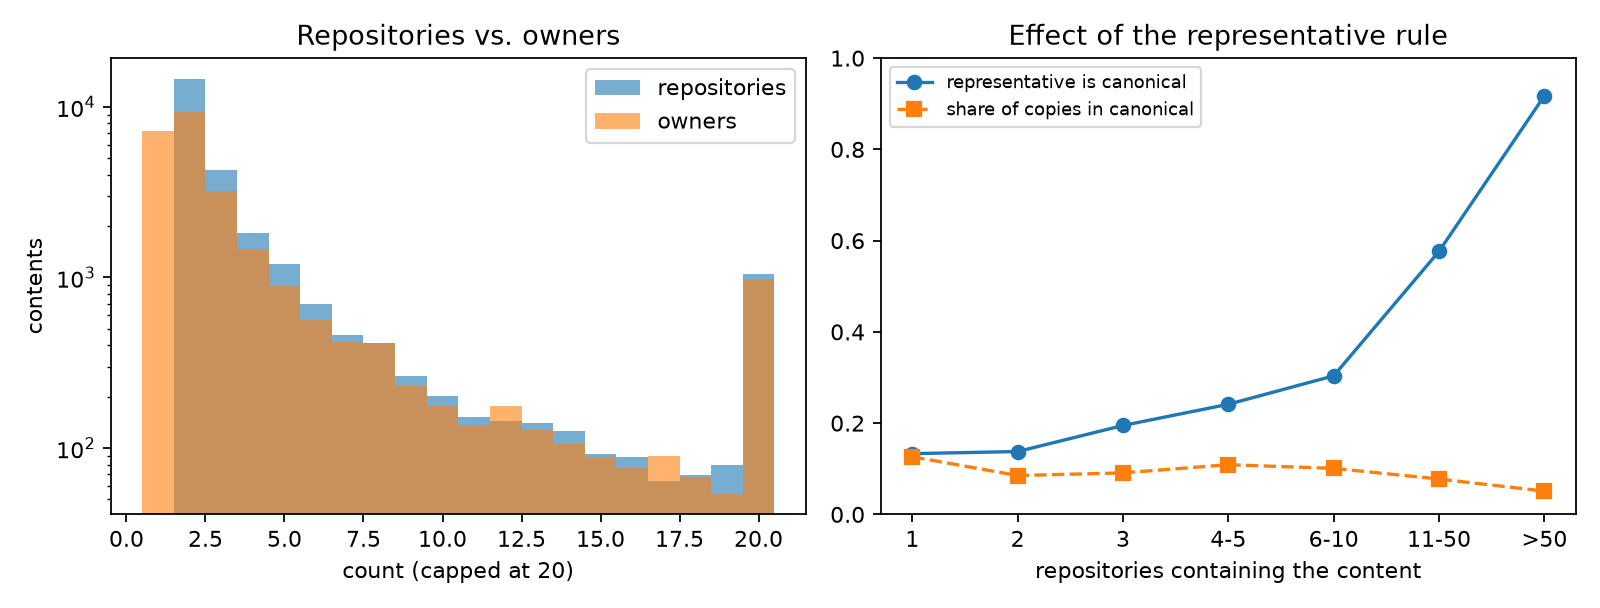
\includegraphics[width=0.82\linewidth]{figures/report_eda_owner_and_selection.png}
\caption{Distributions of repositories and owners (left) and effect of the representative rule (right)}
\label{fig:report-1}
\end{figure}

In the first version of the study, with \texttt{repository\_count} as
target and repository attributes, this inflated the result. With the
Random Forest and the full development set, the repository attributes
gave an RMSLE of 0.575; without \texttt{history\_fetched} and
\texttt{commit\_count}, 0.604 (difference of +0.029, 95\% CI {[}0.018;
0.040{]}), against 0.623 for the mean-of-\texttt{log1p} baseline. The
location of the representative alone (three categories) gave 0.584, and
the history alone 0.594. The ``repository'' view was, to a large extent,
a proxy for location.

\subsection{Main protocol}\label{main-protocol}

With the shortcuts out, 17,733 contents (cap of 50 per owner) and
owner-grouped validation, the results of the Random Forest (RF) and of
the linear models are:

\begin{longtable}[]{@{}
  >{\raggedright\arraybackslash}p{(\linewidth - 8\tabcolsep) * \real{0.1579}}
  >{\raggedleft\arraybackslash}p{(\linewidth - 8\tabcolsep) * \real{0.2105}}
  >{\raggedleft\arraybackslash}p{(\linewidth - 8\tabcolsep) * \real{0.2105}}
  >{\raggedleft\arraybackslash}p{(\linewidth - 8\tabcolsep) * \real{0.2105}}
  >{\raggedleft\arraybackslash}p{(\linewidth - 8\tabcolsep) * \real{0.2105}}@{}}
\caption{Performance by view (mean ± standard deviation over 9
owner-grouped folds).}\tabularnewline
\toprule\noalign{}
\begin{minipage}[b]{\linewidth}\raggedright
View
\end{minipage} & \begin{minipage}[b]{\linewidth}\raggedleft
RF AUC
\end{minipage} & \begin{minipage}[b]{\linewidth}\raggedleft
logistic AUC
\end{minipage} & \begin{minipage}[b]{\linewidth}\raggedleft
RF RMSLE
\end{minipage} & \begin{minipage}[b]{\linewidth}\raggedleft
Ridge RMSLE
\end{minipage} \\
\midrule\noalign{}
\endfirsthead
\toprule\noalign{}
\begin{minipage}[b]{\linewidth}\raggedright
View
\end{minipage} & \begin{minipage}[b]{\linewidth}\raggedleft
RF AUC
\end{minipage} & \begin{minipage}[b]{\linewidth}\raggedleft
logistic AUC
\end{minipage} & \begin{minipage}[b]{\linewidth}\raggedleft
RF RMSLE
\end{minipage} & \begin{minipage}[b]{\linewidth}\raggedleft
Ridge RMSLE
\end{minipage} \\
\midrule\noalign{}
\endhead
\bottomrule\noalign{}
\endlastfoot
skill & 0.660 ± 0.022 & 0.614 & 0.698 ± 0.007 & 0.713 \\
repository & 0.650 ± 0.019 & 0.655 & 0.707 ± 0.011 & 0.702 \\
repository + catalog & 0.666 ± 0.009 & 0.662 & 0.696 ± 0.010 & 0.699 \\
path + catalog & 0.579 ± 0.019 & 0.576 & 0.718 ± 0.018 & 0.714 \\
\textbf{clean (full)} & \textbf{0.716 ± 0.024} & 0.680 & \textbf{0.679 ±
0.011} & 0.694 \\
clean + shortcuts & 0.717 ± 0.022 & 0.682 & 0.637 ± 0.015 & 0.664 \\
shortcuts only & 0.500 ± 0.015 & 0.510 & 0.688 ± 0.010 & 0.693 \\
\emph{baseline} & 0.500 & 0.500 & 0.720 (mean), 0.780 (median) & \\
\end{longtable}

All pre-specified hypotheses are rejected after Holm correction:

\begin{longtable}[]{@{}
  >{\raggedright\arraybackslash}p{(\linewidth - 8\tabcolsep) * \real{0.1875}}
  >{\raggedright\arraybackslash}p{(\linewidth - 8\tabcolsep) * \real{0.1875}}
  >{\raggedright\arraybackslash}p{(\linewidth - 8\tabcolsep) * \real{0.1875}}
  >{\raggedright\arraybackslash}p{(\linewidth - 8\tabcolsep) * \real{0.1875}}
  >{\raggedleft\arraybackslash}p{(\linewidth - 8\tabcolsep) * \real{0.2500}}@{}}
\caption{Pre-specified hypotheses on development (exploratory until the
confirmation of Section 4.7).}\tabularnewline
\toprule\noalign{}
\begin{minipage}[b]{\linewidth}\raggedright
\end{minipage} & \begin{minipage}[b]{\linewidth}\raggedright
Comparison
\end{minipage} & \begin{minipage}[b]{\linewidth}\raggedright
Result
\end{minipage} & \begin{minipage}[b]{\linewidth}\raggedright
95\% CI of the difference
\end{minipage} & \begin{minipage}[b]{\linewidth}\raggedleft
p (Holm)
\end{minipage} \\
\midrule\noalign{}
\endfirsthead
\toprule\noalign{}
\begin{minipage}[b]{\linewidth}\raggedright
\end{minipage} & \begin{minipage}[b]{\linewidth}\raggedright
Comparison
\end{minipage} & \begin{minipage}[b]{\linewidth}\raggedright
Result
\end{minipage} & \begin{minipage}[b]{\linewidth}\raggedright
95\% CI of the difference
\end{minipage} & \begin{minipage}[b]{\linewidth}\raggedleft
p (Holm)
\end{minipage} \\
\midrule\noalign{}
\endhead
\bottomrule\noalign{}
\endlastfoot
H1 & clean RF AUC against 0.5 & 0.716 & +0.216 {[}0.173; 0.259{]} &
\textless{} 0.001 \\
H2 & clean RF RMSLE against the mean & 0.679 vs 0.720 & −0.041
{[}−0.049; −0.033{]} & \textless{} 0.001 \\
H3a & clean against repository+catalog (AUC) & 0.716 vs 0.666 & +0.050
{[}0.017; 0.083{]} & 0.008 \\
H3b & clean against skill (AUC) & 0.716 vs 0.660 & +0.056 {[}0.040;
0.072{]} & \textless{} 0.001 \\
H4 & clean+shortcuts against clean (RMSLE) & 0.637 vs 0.679 & −0.042
{[}−0.055; −0.029{]} & \textless{} 0.001 \\
\end{longtable}

There is a real but modest signal: an AUC of 0.72 and a 6\% reduction in
RMSLE. Skill and repository contribute \textbf{complementarily}: each
block alone sits at AUC 0.65--0.67, and the combination at 0.72 (H3a and
H3b). The shortcuts add to the regression (H4) but, alone, do not
predict cross-owner reuse (AUC 0.50): the regression gain comes from
their correlation with the number of copies, not from cross-owner reuse.
The path, in isolation, barely predicts.

\subsection{Robustness}\label{robustness}

\textbf{Per-owner cap.} The performance of the clean RF changes little
in RMSLE, but a lot in AUC, depending on how concentrated owners are
treated:

\begin{longtable}[]{@{}
  >{\raggedright\arraybackslash}p{(\linewidth - 8\tabcolsep) * \real{0.1579}}
  >{\raggedleft\arraybackslash}p{(\linewidth - 8\tabcolsep) * \real{0.2105}}
  >{\raggedleft\arraybackslash}p{(\linewidth - 8\tabcolsep) * \real{0.2105}}
  >{\raggedleft\arraybackslash}p{(\linewidth - 8\tabcolsep) * \real{0.2105}}
  >{\raggedleft\arraybackslash}p{(\linewidth - 8\tabcolsep) * \real{0.2105}}@{}}
\caption{Sensitivity to the treatment of concentrated owners (RF,
baseline = mean of \texttt{log1p}).}\tabularnewline
\toprule\noalign{}
\begin{minipage}[b]{\linewidth}\raggedright
Treatment
\end{minipage} & \begin{minipage}[b]{\linewidth}\raggedleft
contents
\end{minipage} & \begin{minipage}[b]{\linewidth}\raggedleft
clean RF AUC
\end{minipage} & \begin{minipage}[b]{\linewidth}\raggedleft
RMSLE gain (clean)
\end{minipage} & \begin{minipage}[b]{\linewidth}\raggedleft
gain (shortcuts only)
\end{minipage} \\
\midrule\noalign{}
\endfirsthead
\toprule\noalign{}
\begin{minipage}[b]{\linewidth}\raggedright
Treatment
\end{minipage} & \begin{minipage}[b]{\linewidth}\raggedleft
contents
\end{minipage} & \begin{minipage}[b]{\linewidth}\raggedleft
clean RF AUC
\end{minipage} & \begin{minipage}[b]{\linewidth}\raggedleft
RMSLE gain (clean)
\end{minipage} & \begin{minipage}[b]{\linewidth}\raggedleft
gain (shortcuts only)
\end{minipage} \\
\midrule\noalign{}
\endhead
\bottomrule\noalign{}
\endlastfoot
no limit & 25,918 & 0.747 ± 0.140 & 0.039 & 0.040 \\
exclude owners with more than 1000 & 21,615 & 0.615 ± 0.036 & 0.036 &
0.040 \\
exclude owners with more than 500 & 19,567 & 0.708 ± 0.037 & 0.030 &
0.041 \\
exclude owners with more than 200 & 18,443 & 0.732 ± 0.035 & 0.037 &
0.040 \\
\textbf{50 per owner} & 17,733 & 0.716 ± 0.024 & 0.041 & 0.031 \\
\end{longtable}

The RMSLE is stable (gain of 0.03--0.04), but the AUC oscillates from
0.615 to 0.747: a few owners with 500 to 1000 contents lower the AUC by
0.1, and with no limit a single fold concentrates one owner and the
standard deviation reaches 0.14. Performance therefore depends on the
composition of a dozen accounts. The cap of 50 stabilizes the estimates,
but it is a data-dependent choice.

\textbf{Other checks.} (i) Fixing the location class and training within
each one (owners with more than 500 contents excluded), the clean RF
still beats the baseline: \texttt{canonical} (5,439 contents) RMSLE
−0.141 and AUC 0.714; \texttt{skills-dir} (10,721) −0.013 and 0.672;
\texttt{other} (3,810) −0.011 and 0.828. The signal is not only
location. (ii) With \texttt{repository\_count} as target, the gain of
the clean RF is the same (−0.031 versus −0.030). (iii) Only 18.8\% of
validation rows have a \texttt{name} seen in training; on the subset
without overlap the gain persists (RMSLE −0.039 versus −0.041 on all;
AUC 0.726 versus 0.716), which indicates that variants of the same
\texttt{name} do not explain the result. (iv) Repository-grouped
validation, instead of owner-grouped, did not produce larger estimates
(RMSLE 0.657 versus 0.655; AUC 0.735 versus 0.747, with the standard
deviation of 0.14 of the no-limit case).

\subsection{Interpretation}\label{interpretation}

\begin{figure}[!htbp]
\centering
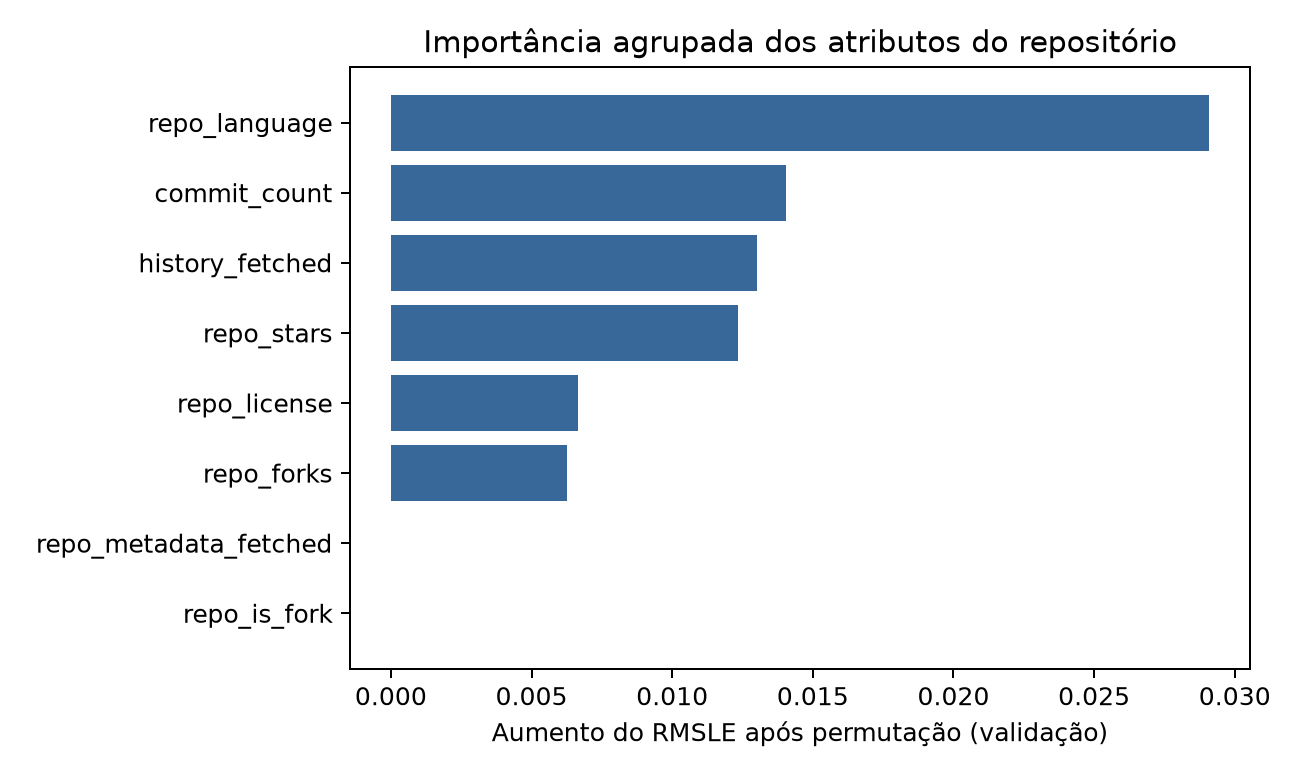
\includegraphics[width=0.82\linewidth]{figures/report_permutation_importance.png}
\caption{Permutation importance of the clean RF (owner-grouped folds; owners with more than 500 contents excluded)}
\label{fig:report-2}
\end{figure}

For cross-owner reuse, the repository block weighs more (AUC drop of
0.104 when permuted) than skill (0.084), catalog (0.016) and path (≈ 0).
Among columns, \texttt{log\_stars} dominates (0.056), followed by
\texttt{log\_forks} (0.021) and push recency (0.016): skills in more
visible repositories are copied more by other owners. In regression,
repository (0.019) and skill (0.018) weigh similarly, and the largest
column is the license (0.013), followed by catalog size (0.011) and path
depth (0.005). We could not identify why the license weighs so much; it
may be an indicator of repositories that clone catalogs. Uncertainties
are large (6 folds), and the correlation among attributes limits the
individual reading.

\subsection{Model selection and
tuning}\label{model-selection-and-tuning}

\begin{longtable}[]{@{}lrrrr@{}}
\caption{Nested validation (mean of 6 outer owner-grouped folds; 6
candidates per search).}\tabularnewline
\toprule\noalign{}
Family & AUC default & AUC searched & RMSLE default & RMSLE searched \\
\midrule\noalign{}
\endfirsthead
\toprule\noalign{}
Family & AUC default & AUC searched & RMSLE default & RMSLE searched \\
\midrule\noalign{}
\endhead
\bottomrule\noalign{}
\endlastfoot
linear & 0.678 & 0.689 & 0.692 & 0.690 \\
KNN & 0.667 & 0.690 & 0.703 & 0.686 \\
tree & 0.614 & 0.634 & 0.807 & 0.699 \\
Random Forest & \textbf{0.716} & 0.701 & 0.679 & 0.675 \\
Gradient Boosting & 0.691 & 0.704 & 0.690 & 0.671 \\
HistGradientBoosting & 0.693 & 0.682 & \textbf{0.670} & 0.688 \\
\emph{baseline} & 0.500 & & 0.720 & \\
\end{longtable}

By the pre-specified rule, we froze the default RF (classification) and
the default HistGradientBoosting (regression). \textbf{The families
tie:} the RF against the runner-up (searched Gradient Boosting) has an
AUC difference of 0.012 (95\% CI {[}−0.003; 0.026{]}), and in regression
the HistGB against the searched Gradient Boosting has −0.001 {[}−0.027;
0.024{]}. Only the decision tree (and, with less evidence, the default
KNN) falls behind, and in classification even these differences do not
survive Holm correction (p between 0.06 and 0.13). The hyperparameter
search did not beat the default configuration (RF classification:
default 0.716 versus searched 0.701).

\subsection{Confirmation on the
holdout}\label{confirmation-on-the-holdout}

The frozen models were evaluated once on 25,011 contents from 10,484
owners disjoint from development.

\begin{longtable}[]{@{}
  >{\raggedright\arraybackslash}p{(\linewidth - 8\tabcolsep) * \real{0.1765}}
  >{\raggedright\arraybackslash}p{(\linewidth - 8\tabcolsep) * \real{0.1765}}
  >{\raggedleft\arraybackslash}p{(\linewidth - 8\tabcolsep) * \real{0.2353}}
  >{\raggedleft\arraybackslash}p{(\linewidth - 8\tabcolsep) * \real{0.2353}}
  >{\raggedright\arraybackslash}p{(\linewidth - 8\tabcolsep) * \real{0.1765}}@{}}
\caption{Single evaluation on the holdout.}\tabularnewline
\toprule\noalign{}
\begin{minipage}[b]{\linewidth}\raggedright
Task
\end{minipage} & \begin{minipage}[b]{\linewidth}\raggedright
Model
\end{minipage} & \begin{minipage}[b]{\linewidth}\raggedleft
Result
\end{minipage} & \begin{minipage}[b]{\linewidth}\raggedleft
Baseline
\end{minipage} & \begin{minipage}[b]{\linewidth}\raggedright
95\% CI (owner bootstrap)
\end{minipage} \\
\midrule\noalign{}
\endfirsthead
\toprule\noalign{}
\begin{minipage}[b]{\linewidth}\raggedright
Task
\end{minipage} & \begin{minipage}[b]{\linewidth}\raggedright
Model
\end{minipage} & \begin{minipage}[b]{\linewidth}\raggedleft
Result
\end{minipage} & \begin{minipage}[b]{\linewidth}\raggedleft
Baseline
\end{minipage} & \begin{minipage}[b]{\linewidth}\raggedright
95\% CI (owner bootstrap)
\end{minipage} \\
\midrule\noalign{}
\endhead
\bottomrule\noalign{}
\endlastfoot
\texttt{cross\_owner} & Random Forest & AUC \textbf{0.731}; PR AUC
0.913; Brier 0.140; log-loss 0.444 & 0.5; 0.808; 0.155; 0.490 & AUC
{[}0.716; 0.745{]}; PR AUC {[}0.905; 0.921{]} \\
\texttt{log1p(owner\_count)} & HistGradientBoosting & RMSLE
\textbf{0.625}; Spearman 0.330 & 0.664 (mean of \texttt{log1p}) &
difference −0.038 {[}−0.044; −0.032{]} \\
\end{longtable}

\begin{figure}[!htbp]
\centering
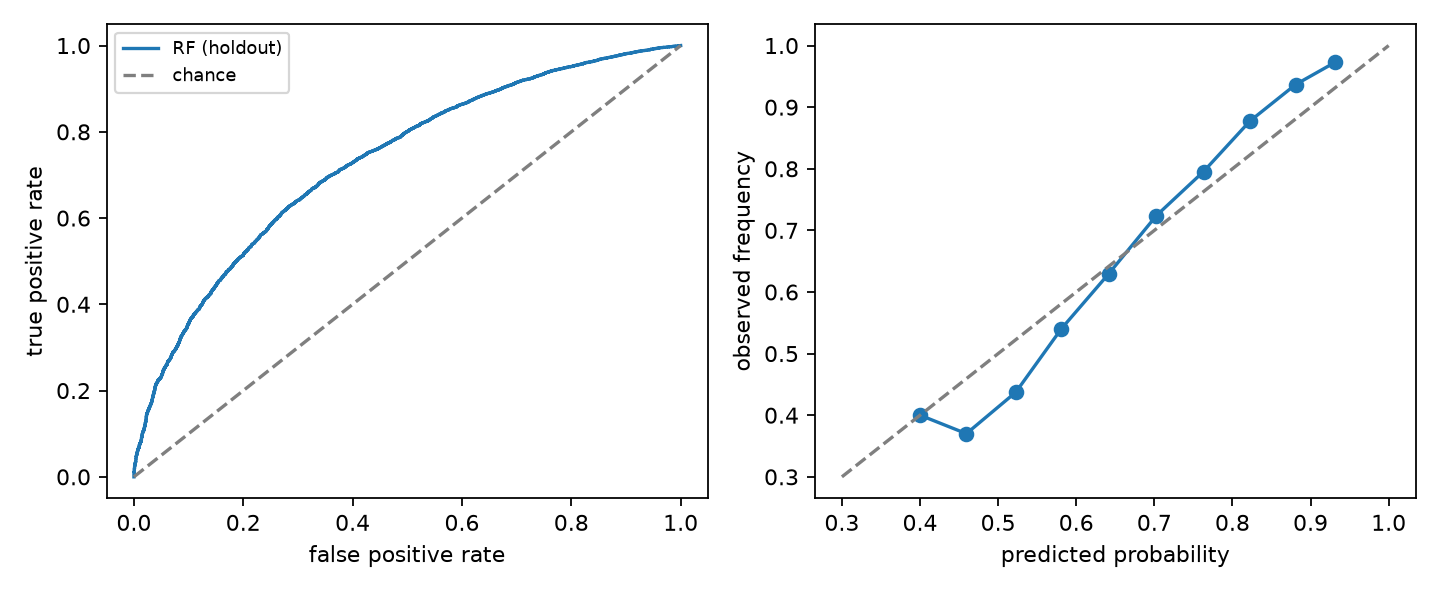
\includegraphics[width=0.82\linewidth]{figures/report_holdout_roc_calibration.png}
\caption{ROC curve and calibration of the RF on the holdout}
\label{fig:report-3}
\end{figure}

The success criteria were met: the lower AUC bound is above 0.5 and the
upper bound of the RMSLE difference is below zero. The holdout AUC
(0.731) is consistent with the nested estimate on development (0.716).
The holdout has a different composition (36\% \texttt{canonical} skills
versus 21\% in development, and 9\% \texttt{other} versus 21\%), since
concentrated owners are left out by construction. H3 and H4 were not
re-evaluated on the holdout and remain exploratory.


\section{Discussão}\label{discussuxe3o}

\subsection{Desempenho e características dos
dados}\label{desempenho-e-caracteruxedsticas-dos-dados}

Os resultados mostram sinal preditivo, mas com alcance limitado. A
representação híbrida teve o menor RMSLE médio do Ridge na validação
interna; a diferença de 0,004 para \texttt{skill-only} é pequena diante
do desvio-padrão entre dobras (0,028 e 0,031). O experimento sugere
informação nos atributos da skill, mas não demonstra superioridade
robusta do híbrido nem desempenho externo de um modelo textual. A maior
correlação de Spearman de \texttt{repository-only} reforça que as
métricas capturam aspectos diferentes.

A assimetria e a sobredispersão do alvo ajudam a explicar o
comportamento. A maioria das skills reutilizadas aparece em poucos
repositórios, enquanto uma parcela pequena concentra contagens elevadas.
A referência constante teve MAE externo menor que o Random Forest (3,067
contra 3,266), embora RMSLE pior (0,714 contra 0,583). Portanto, o ganho
do modelo depende da métrica escolhida. Acima do P95 do treino, o Random
Forest subestimou todas as 324 observações externas, com MAE de 35,15.

\subsection{Comparação dos modelos e vieses
indutivos}\label{comparauxe7uxe3o-dos-modelos-e-vieses-indutivos}

O benchmark completo foi realizado na visão \texttt{repository-only}. O
Random Forest foi escolhido como candidato principal pelo menor RMSLE da
validação agrupada (0,5753). No teste externo, obteve 0,5833; o Gradient
Boosting obteve 0,5907, mas MAE menor (3,1820 contra 3,2663). Esses
valores externos avaliam candidatos já congelados e não são uma nova
rodada de seleção. A variação entre três dobras e a única divisão
externa limitam a precisão de comparações pequenas.

O Ridge impõe uma relação aditiva e regularizada, sendo estável e
relativamente fácil de interpretar, mas tende a encolher valores
extremos. KNN depende da geometria local dos atributos e teve o pior
RMSLE do benchmark completo. A árvore de decisão isolada não superou os
ensembles e apresentou maior variabilidade. Random Forest e Gradient
Boosting capturam não linearidades e interações, mas podem explorar
sinais contextuais que não generalizam para outros ecossistemas.

\subsection{Explicabilidade e
interpretação}\label{explicabilidade-e-interpretauxe7uxe3o}

As análises textuais exploratórias identificaram termos editoriais e
sinais de templates; a robustez ao mascaramento não mostra que sejam
propriedades causais da skill. No Random Forest
\texttt{repository-only}, a importância por impureza destacou
\texttt{repo\_stars}, \texttt{history\_fetched}, ausência de
\texttt{commit\_count} e \texttt{repo\_forks}. Já a permutação agrupada
colocou \texttt{repo\_language} em primeiro (aumento médio de RMSLE
0,029), seguido por \texttt{commit\_count} (0,014),
\texttt{history\_fetched} (0,013) e \texttt{repo\_stars} (0,012). A
divergência decorre em parte das propriedades das medidas de importância
e da correlação entre atributos; o sinal de estrelas variou
substancialmente entre dobras.

No cenário que varia estrelas mantendo as outras entradas, a previsão
média foi não monotônica. Isso enfraquece uma regra simples sobre
popularidade e reutilização, embora o cenário não seja uma estimativa
causal e possa criar combinações raras de atributos. O uso de
\texttt{repo\_language} e histórico também pode codificar origem,
cobertura da coleta ou práticas de distribuição. A interpretação do
Random Forest é apenas contextual; não identifica variáveis textuais ou
estruturais da skill como determinantes da reutilização.

\subsection{Implicações para a engenharia de
software}\label{implicauxe7uxf5es-para-a-engenharia-de-software}

O pipeline pode apoiar análises exploratórias de autoria e descoberta,
indicando convenções que merecem inspeção ou priorizando skills para
auditoria manual. Ele ainda não justifica um linter automático, um
ranking de qualidade ou uma intervenção de autoria. Essas aplicações
exigiriam validação prospectiva, avaliação de utilidade e controle de
possíveis efeitos adversos, como reforçar padrões de popularidade ou
favorecer determinados ecossistemas.

Para o trabalho, a contribuição principal é metodológica: comparar
modelos sob a mesma divisão agrupada, relacionar desempenho a vieses
indutivos e demonstrar que métricas agregadas podem ocultar erros graves
na cauda. Os resultados também delimitam o que pode ser inferido de uma
medida observacional de replicação exata.

\subsection{Ameaças à validade e
limitações}\label{ameauxe7as-uxe0-validade-e-limitauxe7uxf5es}

\texttt{repository\_count} mede a presença de conteúdo idêntico em
repositórios distintos. Não mede intenção de adoção, uso efetivo,
qualidade, utilidade, sucesso de execução ou transferência de
conhecimento. Cópias modificadas e equivalentes semânticos não são
capturados.

O agrupamento por \texttt{representative\_repo\_id} elimina a
sobreposição desse identificador entre treino e validação, mas não
garante que todos os repositórios relacionados, organizações ou cadeias
de cópia estejam separados. Metadados de repositório também podem
funcionar como proxies de popularidade ou origem.

O RMSLE reduz a influência de valores extremos, mas pode ocultar erros
absolutos elevados. Por isso, a análise também utiliza MAE, Spearman,
uma referência constante e auditoria por quantis. A subestimação acima
do P95 mostra que nenhuma métrica isolada caracteriza adequadamente o
desempenho. A comparação textual foi avaliada apenas com Ridge dentro do
desenvolvimento; não autoriza afirmar que o modelo final explica
características intrínsecas da skill.

Os dados provêm de um snapshot específico do GitHub e de um ecossistema
particular de Agent Skills. A generalização para outros períodos, hosts,
comunidades ou mecanismos de distribuição não é garantida. A avaliação
externa reportada é válida para a divisão adotada neste estudo e não
substitui replicações em outros snapshots ou ecossistemas.


\section{Conclusão e trabalhos
futuros}\label{conclusuxe3o-e-trabalhos-futuros}

Este trabalho desenvolveu um pipeline reprodutível para investigar a
intensidade de reutilização de Agent Skills como artefatos de engenharia
de software. A pesquisa modelou o número de repositórios que contêm
exatamente o mesmo \texttt{SKILL.md}, condicionando a análise às skills
reutilizadas. O protocolo combinou atributos estruturais, sinais
textuais e contexto de repositório, utilizou validação agrupada por
\texttt{representative\_repo\_id} e realizou a seleção de atributos
dentro das dobras.

Seis regressores foram comparados sobre 25.918 skills reutilizadas na
visão \texttt{repository-only}. O Random Forest foi escolhido pelo menor
RMSLE médio na validação agrupada (0,5753) e obteve 0,5833 no teste
externo de 6.479 skills. O Gradient Boosting teve MAE externo menor
(3,1820 contra 3,2663). Uma referência constante baseada na mediana do
desenvolvimento teve RMSLE pior (0,7142), mas MAE melhor (3,0665) que o
Random Forest. A escolha do modelo depende, portanto, do objetivo e da
métrica.

A previsão da reutilização é parcial. O Random Forest subestimou todas
as 324 skills do teste acima do P95 do desenvolvimento e teve MAE de
35,15 nessa faixa. O Ridge híbrido apresentou falha semelhante na
validação interna, em análise separada. A comparação das três
representações com Ridge sugere sinal em texto e estrutura, mas a
diferença entre \texttt{hybrid} e \texttt{skill-only} é pequena diante
da variação entre dobras e ainda não foi testada externamente. As
importâncias por permutação do Random Forest se referem a contexto de
repositório, não a propriedades intrínsecas da skill.

Concluímos que características observáveis permitem prever parte da
intensidade de replicação exata entre repositórios, sobretudo na região
central. A evidência não permite explicar por que uma skill se
dissemina, inferir qualidade ou formular uma regra para torná-la mais
reutilizável.

Estudos futuros podem avaliar as representações textuais em um novo
teste externo ainda não consultado, comparar outras estratégias para a
cauda e validar hipóteses em outros snapshots ou ecossistemas. O
presente relatório documenta os resultados e os limites do protocolo
executado.


\bibliographystyle{sbc}

\bibliography{references}

\appendix

\section{Reprodutibilidade e
execução}\label{reprodutibilidade-e-execuuxe7uxe3o}

\subsection{Dados, ambiente e sementes}\label{dados-ambiente-e-sementes}

Fonte pública:
\href{https://huggingface.co/datasets/mvaccargiu/gitskills}{GitSkills no
Hugging Face}, revisão fixa
\texttt{ebab17454a7c236f8f26b183567f1a126f42e3f8} (julho de 2026); o
download verifica SHA-256. O ambiente usa Python 3.12,
\texttt{pyproject.toml} e \texttt{uv.lock}. Sementes: amostragem
\texttt{20261009}; validação 2027, 2028 e 2029; holdout
\texttt{20261110}; bootstrap 2027. A data de referência para idade e
recência é 2026-07-20. A amostra de 200.000 conteúdos é determinística
(\texttt{md5(content\_hash\ \textbar{}\textbar{}\ \textquotesingle{}:20261009\textquotesingle{})}),
não uma amostra aleatória simples. Os comandos partem da raiz do
repositório; \texttt{make} encapsula cada etapa.

\subsection{Construção dos dados e
auditoria}\label{construuxe7uxe3o-dos-dados-e-auditoria}

\begin{verbatim}
uv sync
make data      # download, amostra, divisão e alvo de contagem
make owner     # owner_count, atributos de contexto, auditoria do representante, EDA
\end{verbatim}

Saídas: \texttt{data/processed/owner\_targets.parquet} (contagens por
conteúdo na população completa), \texttt{context\_features.parquet} e,
em \texttt{results/owner/}, \texttt{eda\_summary.json},
\texttt{eda\_target\_quantiles.csv},
\texttt{eda\_owner\_concentration.csv},
\texttt{audit\_by\_repository\_count.csv},
\texttt{audit\_by\_owner\_count.csv}. O manifesto da EDA registra a
concordância da regra do representante (97,2\%).

\subsection{Protocolo principal e
robustez}\label{protocolo-principal-e-robustez}

\begin{verbatim}
make controls     # controle com o desenho original (Seção 4.2)
make primary      # H1–H4 (Seção 4.3), limite de 50 por dono
make robustness   # limiares de donos, classes de localização, alvo alternativo (4.4)
make importance   # importância por permutação (4.5)
\end{verbatim}

\texttt{results/owner/primary/} contém \texttt{primary\_hypotheses.csv},
as tabelas por dobra e os testes pareados exploratórios;
\texttt{results/owner/robustness/} e \texttt{results/owner/models*/}
guardam cada sensibilidade, cada uma com \texttt{manifest.json}.

\subsection{Tuning, congelamento e
holdout}\label{tuning-congelamento-e-holdout}

\begin{verbatim}
make final         # tuning aninhado e congelamento (Seção 4.6); não lê o holdout
make holdout       # constrói o holdout disjunto por dono (Seção 3.9)
make holdout-eval  # avaliação única (Seção 4.7)
\end{verbatim}

Os modelos congelados ficam em
\texttt{results/owner/final/final\_config\_*.json} e foram commitados
antes da avaliação (tag git \texttt{frozen-before-holdout}).
\texttt{holdout-eval} grava
\texttt{results/owner/holdout/evaluation\_lock.json} e \textbf{recusa}
nova execução sem \texttt{-\/-allow-reevaluation}; qualquer reavaliação
deve ser declarada. A reprodução deve conferir
\texttt{holdout\_manifest.json} (sobreposição zero de donos e de
conteúdos).

\subsection{Mapa entre tabelas, figuras e
artefatos}\label{mapa-entre-tabelas-figuras-e-artefatos}

\begin{longtable}[]{@{}
  >{\raggedright\arraybackslash}p{(\linewidth - 2\tabcolsep) * \real{0.5000}}
  >{\raggedright\arraybackslash}p{(\linewidth - 2\tabcolsep) * \real{0.5000}}@{}}
\caption{Origem dos números do relatório.}\tabularnewline
\toprule\noalign{}
\begin{minipage}[b]{\linewidth}\raggedright
Item
\end{minipage} & \begin{minipage}[b]{\linewidth}\raggedright
Artefato
\end{minipage} \\
\midrule\noalign{}
\endfirsthead
\toprule\noalign{}
\begin{minipage}[b]{\linewidth}\raggedright
Item
\end{minipage} & \begin{minipage}[b]{\linewidth}\raggedright
Artefato
\end{minipage} \\
\midrule\noalign{}
\endhead
\bottomrule\noalign{}
\endlastfoot
Distribuição e concentração (4.1) &
\texttt{results/owner/eda\_target\_quantiles.csv},
\texttt{eda\_owner\_concentration.csv} \\
Viés do representante (4.2, figura) &
\texttt{results/owner/audit\_by\_repository\_count.csv},
\texttt{eda\_owner\_and\_selection.png} \\
Controle com o desenho original (4.2) &
\texttt{results/controls/shortcut\_summary.csv},
\texttt{shortcut\_paired.csv} \\
Visões e hipóteses (4.3) &
\texttt{results/owner/primary/\{classification,regression\}\_summary.csv},
\texttt{primary\_hypotheses.csv} \\
Sensibilidade (4.4) &
\texttt{results/owner/figures/sensitivity\_owner\_limit.csv},
\texttt{results/owner/robustness/*} \\
Importância (4.5) &
\texttt{results/owner/importance/*\_importance.csv} \\
Tuning (4.6) & \texttt{results/owner/final/*\_nested\_summary.csv},
\texttt{*\_selection\_tests.csv} \\
Holdout (4.7) & \texttt{results/owner/holdout/holdout\_results.json} \\
\end{longtable}

\subsection{Verificações, desvios e
limites}\label{verificauxe7uxf5es-desvios-e-limites}

\begin{verbatim}
make test
\end{verbatim}

Os testes cobrem a exclusão de atributos contaminados, os padrões de
caminho, os testes pareados e a correção de Holm, o bootstrap por dono e
a disjunção do holdout. Desvios em relação ao protocolo: tuning com 2×3
dobras e 6 candidatas (planejado 3×3 e 12) por custo computacional; a
máquina de desenvolvimento tinha 8 GB de memória. Resultados numéricos
podem variar nas últimas casas com versões diferentes das bibliotecas. A
primeira versão do estudo (alvo \texttt{repository\_count}, teste
externo original) permanece no repositório
(\texttt{results/count\_regression},
\texttt{results/discipline\_benchmark}) apenas como histórico, e não
sustenta nenhuma conclusão deste relatório.


\section{Uso de ferramentas de inteligência
artificial}\label{uso-de-ferramentas-de-inteliguxeancia-artificial}

OpenAI Codex \cite{openai_codex} foi utilizado para planejar o pipeline, auxiliar na
implementação e depuração do código, organizar e revisar o texto e
conferir a consistência entre tabelas e resultados. O autor definiu os
alvos e as restrições da pesquisa, examinou os artefatos produzidos e é
responsável pelo código, pelas afirmações e pela interpretação final. A
ferramenta deve ser citada na versão formatada do artigo conforme a
orientação da disciplina.

O \texttt{registro\ de\ uso} resume as tarefas, mas não preserva todos
os prompts e respostas integrais. O \texttt{suplemento\ de\ IA} contém
cinco prompts verbatim disponíveis no histórico, incluindo o pedido
desta revisão, e explicita a incompletude do registro. Não foram
inventados prompts de sessões de implementação ausentes. Erros
relevantes de assistência incluíram risco de transportar conclusões do
pipeline binário para a regressão, confundir associação com causalidade
e tratar a avaliação externa como seleção. As afirmações quantitativas
deste relatório foram reconciliadas com os CSVs e manifestos mencionados
no Apêndice A; a bibliografia ainda requer conferência editorial final
antes da submissão.


\end{document}
